\documentclass[aspectratio=169, 10pt]{beamer}

% =========================================================================
% MINIMALIST BEIGE & NAVY THEME (MARP / PROJECT PROPOSAL STYLE)
% Custom crafted to match the user's visual identity:
% Background: #F3EBE1 (Warm Cream Beige)
% Typography & Elements: #262E5B (Deep Indigo Navy)
% Signature: Right-edge vertical Navy bar with rounded inner corners
% =========================================================================

\usetheme{default}
\setbeamertemplate{navigation symbols}{}
\setbeamertemplate{headline}{}
\setbeamertemplate{footline}{}

\usepackage{fontspec}
\setsansfont{Segoe UI}
\setmainfont{Segoe UI}

\usepackage{graphicx}
\usepackage{booktabs}
\usepackage{amsmath,amssymb}
\usepackage{xcolor}
\usepackage{tikz}
\usetikzlibrary{calc,positioning,shapes.geometric,arrows.meta}

% --- COLOR DEFINITIONS ---
\definecolor{bgBeige}{RGB}{243, 235, 225}    % #F3EBE1 - Warm Beige Canvas
\definecolor{navyMain}{RGB}{38, 46, 91}      % #262E5B - Deep Indigo Navy
\definecolor{navyMuted}{RGB}{85, 95, 140}    % Muted Navy for subtext/metadata
\definecolor{navyLight}{RGB}{228, 225, 235}  % Soft tinted fill
\definecolor{accentDark}{RGB}{185, 28, 28}   % Alert crimson

\setbeamercolor{background canvas}{bg=bgBeige}
\setbeamercolor{normal text}{fg=navyMain}
\setbeamercolor{structure}{fg=navyMain}

% Set margins so text never touches the right navy bar
\setbeamersize{text margin left=1.0cm, text margin right=1.8cm}

% --- SIGNATURE BACKGROUND WITH RIGHT NAVY ACCENT BAR ---
\setbeamertemplate{background}{
    \begin{tikzpicture}[remember picture,overlay]
        % Base Beige Canvas
        \fill[bgBeige] (current page.south west) rectangle (current page.north east);
        % Right vertical navy bar with 2 rounded inside corners (top-left & bottom-left)
        \fill[navyMain, rounded corners=16pt] 
            ($(current page.north east)+(-1.05cm, 0)$) rectangle ($(current page.south east)+(1.0cm, 0)$);
    \end{tikzpicture}
}

% --- CUSTOM SLIDE HEADER ---
\newcommand{\slideheader}[2]{%
    \vspace*{-0.15cm}%
    {\fontsize{7.5pt}{9pt}\selectfont \textbf{\color{navyMuted}\MakeUppercase{#1}}}\\[0.03cm]
    {\fontsize{13.5pt}{16pt}\selectfont \textbf{\color{navyMain}\MakeUppercase{#2}}}\\[0.08cm]
}

% --- CUSTOM FOOTER NUMBER ---
\newcommand{\slidenumber}[1]{%
    \begin{tikzpicture}[remember picture,overlay]
        \node[anchor=south east] at ($(current page.south east)+(-1.4cm, 0.35cm)$) {
            \textcolor{navyMuted}{\fontsize{8.5pt}{10pt}\selectfont \textbf{\insertframenumber}}
        };
        \node[anchor=south west] at ($(current page.south west)+(1.0cm, 0.35cm)$) {
            \textcolor{navyMuted}{\fontsize{7pt}{8pt}\selectfont \textit{Hands-On Data Visualization} -- Jack Dougherty \& Ilya Ilyankou}
        };
    \end{tikzpicture}%
}

% --- PILL BOX MACRO ---

\definecolor{boxBg}{RGB}{230, 221, 208}      % Tinted card bg #E6DDD0
\definecolor{accentRed}{RGB}{185, 28, 28}    % Alert crimson #B91C1C

\newcommand{\calloutbox}[3][\textwidth]{%
    \begin{tikzpicture}
        \node[
            fill=boxBg,
            draw=navyMain,
            line width=0.8pt,
            rounded corners=4pt,
            inner sep=5pt,
            text width=#1-14pt,
            align=left
        ] {
            {\fontsize{8.5pt}{10.5pt}\selectfont \textbf{\color{navyMain}#2}}\\[0.03cm]
            {\fontsize{7.5pt}{9.5pt}\selectfont \color{navyMain}#3}
        };
    \end{tikzpicture}%
}

\newcommand{\pillbox}[2][]{%
    \begin{tikzpicture}
        \node[
            draw=navyMain,
            rounded corners=10pt,
            line width=1.1pt,
            inner xsep=12pt,
            inner ysep=4pt,
            text=navyMain,
            #1
        ] {\textbf{#2}};
    \end{tikzpicture}%
}

\begin{document}


\begin{frame}[plain, c]


\begin{tikzpicture}[remember picture,overlay]
    \node[anchor=north west] at ($(current page.north west)+(1.0cm, -0.8cm)$) {
        \textcolor{navyMuted}{\fontsize{8.5pt}{10.5pt}\selectfont Tháng 10, 2026}
    };
    \node[anchor=west, text width=0.76\textwidth] at ($(current page.west)+(1.0cm, 0.3cm)$) {
        {\fontsize{13pt}{15pt}\selectfont \textbf{\color{navyMuted} PHẦN 4 • BÁO CÁO CHUYÊN ĐỀ}}\\[0.25cm]
        {\fontsize{28pt}{32pt}\selectfont \textbf{\color{navyMain} ĐẠO ĐỨC DỮ LIỆU \&}}\\[0.12cm]
        {\fontsize{20pt}{24pt}\selectfont \textbf{\color{navyMain} NGHỆ THUẬT KỂ CHUYỆN}}\\[0.35cm]
        \pillbox{\fontsize{9.5pt}{11.5pt}\selectfont Phát Hiện Sự Lừa Dối, Giảm Định Kiến \& Thúc Đẩy Hành Động (Chương 14, 15)}\\[0.45cm]
        {\fontsize{8.5pt}{10.5pt}\selectfont \color{navyMuted} Thuyết trình: \textbf{Người 4} • Tác phẩm: \textit{Hands-On Data Visualization} (Jack Dougherty \& Ilya Ilyankou)}
    };
\end{tikzpicture}
\slidenumber{01}
\end{frame}

% ==================== SLIDE 2: MỤC LỤC PHẦN 4 ====================


\begin{frame}[plain, t]


\slideheader{Phần 4 • Tổng Quan}{Nội Dung Trình Bày (Our Contents)}
\begin{columns}[T]
\begin{column}{0.31\textwidth}
\begin{tikzpicture}
    \node[draw=navyMain, fill=boxBg, rounded corners=6pt, line width=0.9pt, inner sep=7pt, text width=\textwidth-16pt, align=left] {
        {\fontsize{9.5pt}{11.5pt}\selectfont \textbf{\color{navyMain} 01. CHƯƠNG 14 (A)}}\\[0.05cm]
        {\fontsize{8pt}{9.5pt}\selectfont \textbf{\color{navyMuted} Phát Hiện Lừa Dối}}\\[0.15cm]
        {\fontsize{7.2pt}{9pt}\selectfont \color{navyMain}
        • 3 phân loại: Sai, Lừa, Thật\\
        • Cắt trục tung: GDP \& Nhiệt độ\\
        • Méo khung hình Aspect Ratio\\
        • Bẫy 2 trục tung \& Connected Scatter\\
        • 2 bản đồ đối lập cùng trung thực}
    };
\end{tikzpicture}
\end{column}
\begin{column}{0.31\textwidth}
\begin{tikzpicture}
    \node[draw=navyMain, fill=boxBg, rounded corners=6pt, line width=0.9pt, inner sep=7pt, text width=\textwidth-16pt, align=left] {
        {\fontsize{9.5pt}{11.5pt}\selectfont \textbf{\color{navyMain} 02. CHƯƠNG 14 (B)}}\\[0.05cm]
        {\fontsize{8pt}{9.5pt}\selectfont \textbf{\color{navyMuted} Giảm Thiểu Định Kiến}}\\[0.15cm]
        {\fontsize{7.2pt}{9pt}\selectfont \color{navyMain}
        • Nhận thức: Xác nhận \& Đóng khung\\
        • Thuật toán: COMPAS, Apple Card\\
        • Định kiến liên nhóm Urban Inst.\\
        • Không gian: Diện tích \& Mercator\\
        • Giải pháp Cartogram \& Loại trừ}
    };
\end{tikzpicture}
\end{column}
\begin{column}{0.31\textwidth}
\begin{tikzpicture}
    \node[draw=navyMain, fill=boxBg, rounded corners=6pt, line width=0.9pt, inner sep=7pt, text width=\textwidth-16pt, align=left] {
        {\fontsize{9.5pt}{11.5pt}\selectfont \textbf{\color{navyMain} 03. CHƯƠNG 15}}\\[0.05cm]
        {\fontsize{8pt}{9.5pt}\selectfont \textbf{\color{navyMuted} Kể Chuyện Dữ Liệu}}\\[0.15cm]
        {\fontsize{7.2pt}{9pt}\selectfont \color{navyMain}
        • Công thức: Tell -- Show -- Why\\
        • Phân cảnh Data Storyboard\\
        • Nhấn mạnh màu \& Chú thích (Nhựa)\\
        • Minh bạch sự bất định (Nét đứt)\\
        • Định dạng: Web, Screencast, Walk}
    };
\end{tikzpicture}
\end{column}
\end{columns}
\slidenumber{02}
\end{frame}

% ==================== SLIDE 3: CHUYỂN TIẾP MỤC 01 ====================


\begin{frame}[plain, c]


\begin{tikzpicture}[remember picture,overlay]
    \node[anchor=west, text width=0.76\textwidth] at ($(current page.west)+(1.0cm, 0.2cm)$) {
        {\fontsize{13pt}{15pt}\selectfont \textbf{\color{navyMuted} PHẦN 4 • MỤC 01}}\\[0.25cm]
        {\fontsize{28pt}{32pt}\selectfont \textbf{\color{navyMain} PHÁT HIỆN ``SỰ LỪA DỐI''}}\\[0.12cm]
        {\fontsize{22pt}{26pt}\selectfont \textbf{\color{navyMain} TRONG ĐỒ THỊ}}\\[0.35cm]
        \pillbox{\fontsize{10pt}{12pt}\selectfont Chapter 14: Detect Lies in Charts and Maps}\\[0.45cm]
        {\normalsize \color{navyMuted} \textit{``Muốn bắt kẻ gian, trước hết phải hiểu mánh khóe của kẻ gian.''}}
    };
\end{tikzpicture}
\slidenumber{03}
\end{frame}

% ==================== SLIDE 4: 3 PHÂN LOẠI TRỰC QUAN HÓA ====================


\begin{frame}[plain, t]


\slideheader{Mục 01 • Phát Hiện Lừa Dối}{3 Phân Loại: Sai (Wrong), Đánh Lừa \& Trung Thực}
\begin{columns}[T]
\begin{column}{0.31\textwidth}
\calloutbox[\textwidth]{1. Sai (Wrong)}{
    • Bóp méo số liệu thực tế hoặc \textbf{vi phạm trực tiếp quy tắc thiết kế cứng}.\\[0.1cm]
    • \textit{Ví dụ:} Biểu đồ cột không bắt đầu từ 0 (Truncated baseline), hoặc biểu đồ tròn có tổng các phần $\neq 100\%$.
}
\end{column}
\begin{column}{0.31\textwidth}
\calloutbox[\textwidth]{2. Đánh Lừa (Misleading)}{
    • Số liệu hoàn toàn chính xác, \textbf{không vi phạm quy tắc kỹ thuật}, nhưng cố tình bóp méo hình thái hiển thị.\\[0.1cm]
    • \textit{Ví dụ:} Kéo giãn trục tung quá mức hoặc méo tỷ lệ khung hình (Aspect Ratio) trên biểu đồ đường.
}
\end{column}
\begin{column}{0.31\textwidth}
\calloutbox[\textwidth]{3. Trung Thực (Truthful)}{
    • Hiển thị dữ liệu chính xác, tuân thủ nguyên tắc thị giác.\\[0.1cm]
    • \textbf{Lưu ý:} Có thể có \textbf{nhiều hơn một cách biểu diễn trung thực} cho cùng 1 bộ dữ liệu tùy theo góc nhìn muốn làm nổi bật.
}
\end{column}
\end{columns}
\slidenumber{04}
\end{frame}

% ==================== SLIDE 5: MÁNH KHÓE 1: PHÓNG ĐẠI & THU NHỎ TRỤC TUNG ====================


\begin{frame}[plain, t]


\slideheader{Mục 01 • Phát Hiện Lừa Dối}{Mánh Khóe 1: Thao Túng Điểm Đầu/Cuối Trục Tung}
\begin{columns}[T]
\begin{column}{0.52\textwidth}
{\fontsize{7.8pt}{9.8pt}\selectfont
\textbf{A. Phóng đại sự thay đổi -- Cắt cụt gốc 0 (GDP Mỹ)}
\begin{itemize}\setlength{\itemsep}{1pt}
    \item GDP tăng nhẹ $0,96\%$ (từ $\$21,54\text{T}$ lên $\$21,75\text{T}$).
    \item Cắt trục tại $\$21.500\text{T}$ làm cột sau \textbf{cao gấp 5 lần} cột trước! $\rightarrow$ \textcolor{accentRed}{\textbf{SAI (Wrong)}} vì vi phạm gốc 0 của biểu đồ cột.
\end{itemize}

\vspace{0.08cm}
\textbf{B. Làm lu mờ biến động -- Kéo dài trục tung (Nhiệt độ)}
\begin{itemize}\setlength{\itemsep}{1pt}
    \item Nhiệt độ Trái Đất tăng $+1^\circ\text{C}$ (nguy cơ tan băng).
    \item Kẻ phủ nhận kéo trục $[-5^\circ\text{C}, +5^\circ\text{C}]$ làm đường bẹp dí nằm ngang! $\rightarrow$ \textbf{ĐÁNH LỪA (Misleading)}.
\end{itemize}
}
\end{column}
\begin{column}{0.44\textwidth}
\centering
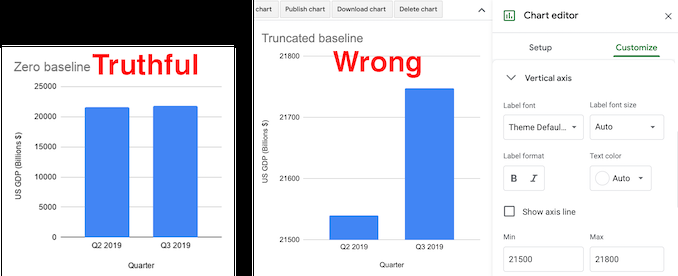
\includegraphics[width=\textwidth, height=0.22\textheight, keepaspectratio]{images/fig_14_1_truncated_gdp.png}\\[0.08cm]
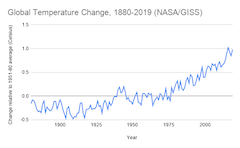
\includegraphics[width=0.48\textwidth, height=0.22\textheight, keepaspectratio]{images/fig_14_2_temperature_default.png}
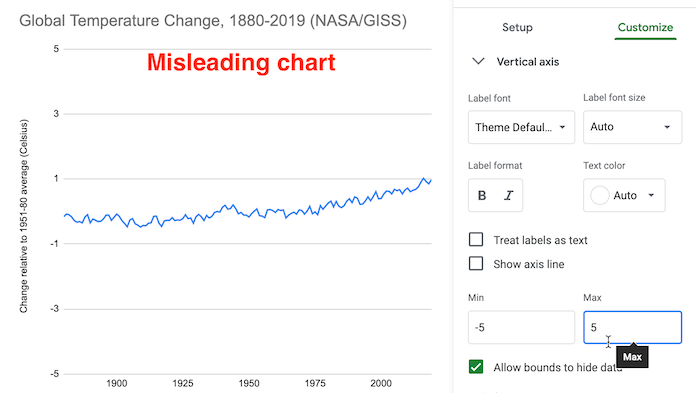
\includegraphics[width=0.48\textwidth, height=0.22\textheight, keepaspectratio]{images/fig_14_3_temperature_flattened.png}\\[0.08cm]
{\fontsize{6.5pt}{7.8pt}\selectfont \textcolor{navyMuted}{\textit{Hình 14.1: Cắt trục GDP \& Hình 14.2, 14.3: Ép bẹp đường nhiệt độ.}}}
\end{column}
\end{columns}
\slidenumber{05}
\end{frame}

% ==================== SLIDE 6: MÁNH KHÓE 2: BÓP MÉO TỶ LỆ KHUNG HÌNH ====================


\begin{frame}[plain, t]


\slideheader{Mục 01 • Phát Hiện Lừa Dối}{Mánh Khóe 2: Bóp Méo Tỷ Lệ Khung Hình (Aspect Ratio)}
\begin{columns}[T]
\begin{column}{0.52\textwidth}
{\fontsize{8.2pt}{10.5pt}\selectfont
\textbf{Tỷ lệ khung hình = Chiều rộng / Chiều cao ($\text{W} : \text{H}$):}

\vspace{0.12cm}
\textbf{1. Kéo giãn chiều ngang quá mức ($5.7 : 1$):}
\begin{itemize}\setlength{\itemsep}{1.5pt}
    \item Đồ thị NASA từ $1.6:1$ bị kéo bẹt thành $5.7:1$ $\rightarrow$ Độ dốc biến mất, tạo ảo giác khí hậu hoàn toàn ổn định!
\end{itemize}

\vspace{0.12cm}
\textbf{2. Nghịch lý khi áp dụng máy móc quy tắc Alberto Cairo:}
\begin{itemize}\setlength{\itemsep}{1.5pt}
    \item \textit{Tính theo mức tăng biến thiên ($300\% = 3/1$):} Khung hình $1:3$ \textbf{cao vút như tòa tháp}, phóng đại quá đà!
    \item \textit{Tính theo nhiệt độ tuyệt đối ($8\% \approx 1/12$):} Khung hình $12:1$ \textbf{dẹt mỏng như sợi chỉ}, che lấp hoàn toàn thảm họa!
\end{itemize}
}
\end{column}
\begin{column}{0.44\textwidth}
\centering
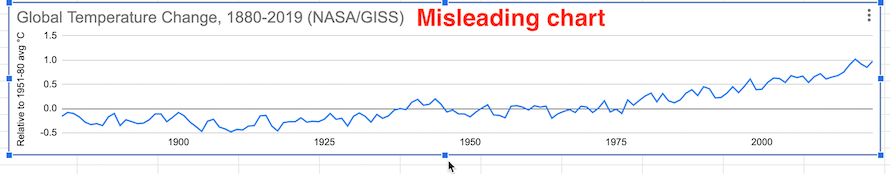
\includegraphics[width=\textwidth, height=0.15\textheight, keepaspectratio]{images/fig_14_4_aspect_ratio_stretched.png}\\[0.08cm]
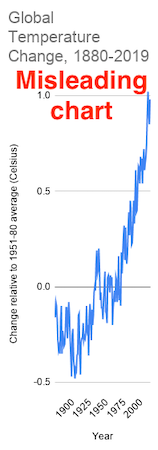
\includegraphics[width=0.35\textwidth, height=0.3\textheight, keepaspectratio]{images/fig_14_5_aspect_ratio_tall.png}
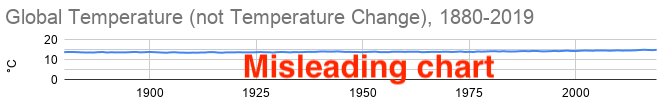
\includegraphics[width=0.6\textwidth, height=0.15\textheight, keepaspectratio]{images/fig_14_6_aspect_ratio_flat.png}\\[0.08cm]
{\fontsize{6.5pt}{7.8pt}\selectfont \textcolor{navyMuted}{\textit{Hình 14.4 (5.7:1), Hình 14.5 (1:3 cao vút), Hình 14.6 (12:1 sợi chỉ).}}}
\end{column}
\end{columns}
\slidenumber{06}
\end{frame}

% ==================== SLIDE 7: MÁNH KHÓE 3: BẪY BIỂU ĐỒ HAI TRỤC TUNG ====================


\begin{frame}[plain, t]


\slideheader{Mục 01 • Phát Hiện Lừa Dối}{Mánh Khóe 3: Cái Bẫy Biểu Đồ Hai Trục Tung}
\begin{columns}[T]
\begin{column}{0.52\textwidth}
{\fontsize{7.8pt}{9.8pt}\selectfont
\textbf{Case Study: Nhiệt độ Toàn cầu \& GDP Mỹ (1929--2019)}

\vspace{0.08cm}
\textbf{3 tầng thao túng tâm lý trong Figure 14.9:}
\begin{enumerate}\setlength{\itemsep}{1pt}
    \item \textit{Thang đo vô lý:} Ép nhiệt độ bẹp dưới đáy, GDP vút cao $\rightarrow$ Ảo giác kinh tế tăng rực rỡ còn khí hậu không đổi.
    \item \textit{Dữ liệu không tương đương:} Dùng GDP danh nghĩa chưa điều chỉnh lạm phát.
    \item \textit{Màu sắc ngược nghĩa:} Xanh mát cho nhiệt độ nóng, đỏ cho GDP!
\end{enumerate}

\vspace{0.08cm}
\textbf{✅ Giải pháp: Connected Scatter Chart (Figure 14.10)}
\begin{itemize}\setlength{\itemsep}{1pt}
    \item Trục hoành là \textbf{GDP thực}, trục tung là \textbf{Mức tăng nhiệt độ}.
    \item Thấy rõ: Kinh tế tăng kéo theo biến đổi khí hậu!
\end{itemize}
}
\end{column}
\begin{column}{0.44\textwidth}
\centering
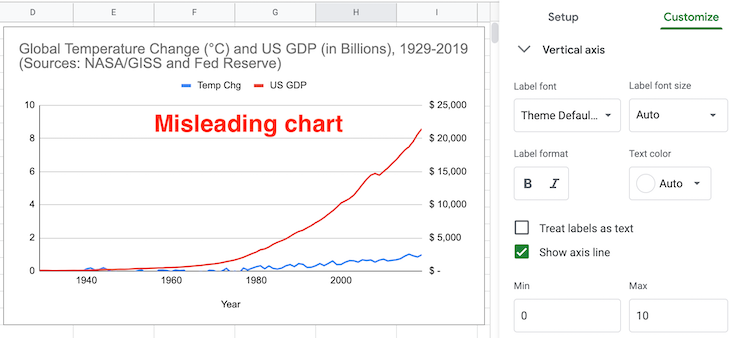
\includegraphics[width=\textwidth, height=0.23\textheight, keepaspectratio]{images/fig_14_9_dual_axis_misleading.png}\\[0.1cm]
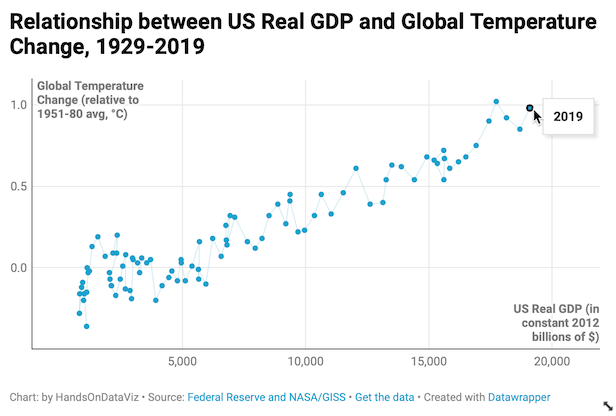
\includegraphics[width=\textwidth, height=0.24\textheight, keepaspectratio]{images/fig_14_10_connected_scatter.png}\\[0.08cm]
{\fontsize{6.5pt}{7.8pt}\selectfont \textcolor{navyMuted}{\textit{Hình 14.9: Hai trục tung lừa dối vs Hình 14.10: Connected scatter trung thực.}}}
\end{column}
\end{columns}
\slidenumber{07}
\end{frame}

% ==================== SLIDE 8: HAI BẢN ĐỒ ĐỐI LẬP CÙNG TRUNG THỰC ====================


\begin{frame}[plain, t]


\slideheader{Mục 01 • Phát Hiện Lừa Dối}{Hai Bản Đồ Đối Lập Nhưng Cùng Trung Thực!}
\begin{columns}[T]
\begin{column}{0.52\textwidth}
{\fontsize{7.8pt}{9.8pt}\selectfont
\textbf{Dữ liệu Bất bình đẳng thu nhập (Top 1\% giàu nhất):}
Mỹ chiếm \textbf{20,5\%}, Brazil chiếm \textbf{28,3\%}.

\vspace{0.1cm}
\begin{table}[h]
\centering
\begin{tabular}{p{0.45\textwidth} p{0.45\textwidth}}
\toprule
\textbf{\color{navyMain} Bản đồ 1 (Linear)} & \textbf{\color{navyMain} Bản đồ 2 (Jenks 3 Steps)} \\
\midrule
Xếp thẳng từ $5\%$ đến $31\%$. & Chia 3 nhóm tự nhiên. \\
Mỹ ($20,5\%$) màu \textbf{xanh trung bình}, trông ôn hòa giống đa số các nước. & Mỹ rơi vào nhóm cao nhất ($\ge 19\%$) với \textbf{màu xanh đậm nhất} cùng Brazil, Nga! \\
\bottomrule
\end{tabular}
\end{table}

\vspace{-0.1cm}
\calloutbox[\textwidth]{Giải Mã Bằng Histogram (Figure 14.14)}{
    Cả hai đều đúng! Mỹ nằm ở giữa khoảng cách số học min--max, nhưng lại nằm ở nhóm đầu xét theo mật độ phân cụm thế giới.
}
}
\end{column}
\begin{column}{0.44\textwidth}
\centering
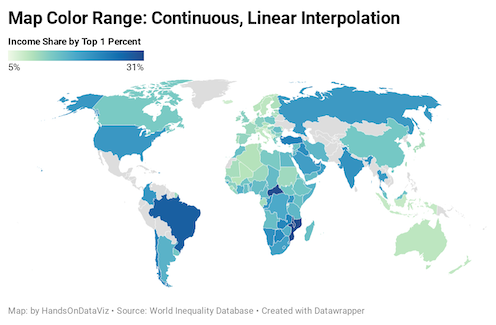
\includegraphics[width=0.48\textwidth, height=0.22\textheight, keepaspectratio]{images/fig_14_12_inequality_continuous.png}
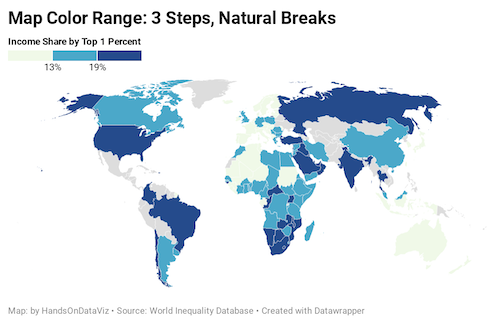
\includegraphics[width=0.48\textwidth, height=0.22\textheight, keepaspectratio]{images/fig_14_13_inequality_jenks.png}\\[0.08cm]
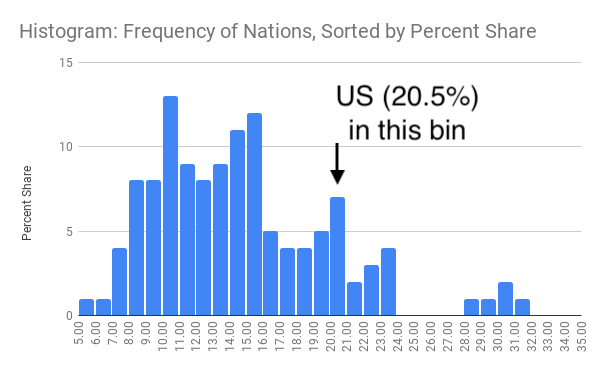
\includegraphics[width=\textwidth, height=0.24\textheight, keepaspectratio]{images/fig_14_14_inequality_histogram.png}\\[0.08cm]
{\fontsize{6.5pt}{7.8pt}\selectfont \textcolor{navyMuted}{\textit{Hình 14.12: Linear; Hình 14.13: Jenks; Hình 14.14: Histogram giải mã.}}}
\end{column}
\end{columns}
\slidenumber{08}
\end{frame}

% ==================== SLIDE 9: CHUYỂN TIẾP MỤC 02 ====================


\begin{frame}[plain, c]


\begin{tikzpicture}[remember picture,overlay]
    \node[anchor=west, text width=0.76\textwidth] at ($(current page.west)+(1.0cm, 0.2cm)$) {
        {\fontsize{13pt}{15pt}\selectfont \textbf{\color{navyMuted} PHẦN 4 • MỤC 02}}\\[0.25cm]
        {\fontsize{28pt}{32pt}\selectfont \textbf{\color{navyMain} NHẬN DIỆN \& GIẢM THIỂU}}\\[0.12cm]
        {\fontsize{22pt}{26pt}\selectfont \textbf{\color{navyMain} ĐỊNH KIẾN (BIAS)}}\\[0.35cm]
        \pillbox{\fontsize{10pt}{12pt}\selectfont Recognize and Reduce Data \& Spatial Bias}\\[0.45cm]
        {\normalsize \color{navyMuted} \textit{``Từ định kiến nhận thức, thuật toán\\cho tới định kiến bản đồ học.''}}
    };
\end{tikzpicture}
\slidenumber{09}
\end{frame}

% ==================== SLIDE 10: 4 ĐỊNH KIẾN DỮ LIỆU (1): NHẬN THỨC ====================


\begin{frame}[plain, t]


\slideheader{Mục 02 • Giảm Thiểu Định Kiến}{Định Kiến Nhận Thức (Cognitive Biases)}
\begin{columns}[T]
\begin{column}{0.31\textwidth}
\calloutbox[\textwidth]{1. Thiên Vị Xác Nhận}{
    \textbf{Confirmation bias:}\\[0.05cm]
    • Não bộ chỉ tìm và tin dữ liệu khớp với định kiến có sẵn.\\[0.1cm]
    $\rightarrow$ \textbf{Khắc phục:} Chủ động tìm kiếm dữ liệu và cách diễn giải phản biện lại giả thuyết của mình.
}
\end{column}
\begin{column}{0.31\textwidth}
\calloutbox[\textwidth]{2. Thiên Vị Khuôn Mẫu}{
    \textbf{Pattern bias:}\\[0.05cm]
    • Não người luôn cố tìm quy luật ngay cả trong các con số ngẫu nhiên (nhiễu/noise).\\[0.1cm]
    $\rightarrow$ \textbf{Khắc phục:} Bắt buộc sử dụng kiểm định ý nghĩa thống kê trước khi kết luận.
}
\end{column}
\begin{column}{0.31\textwidth}
\calloutbox[\textwidth]{3. Thiên Vị Đóng Khung}{
    \textbf{Framing bias (Spiegelhalter):}\\[0.05cm]
    • \textit{``Tỷ lệ tử vong 5\%''} nghe đáng sợ hơn nhiều so với \textit{``Tỷ lệ sống sót 95\%''}.\\[0.08cm]
    • Nói thêm: \textit{``20 trên 400 người chết''} gây ám ảnh vì não hình dung ra con người cụ thể.
}
\end{column}
\end{columns}
\slidenumber{10}
\end{frame}

% ==================== SLIDE 11: 4 ĐỊNH KIẾN (2): THUẬT TOÁN & LIÊN NHÓM ====================


\begin{frame}[plain, t]


\slideheader{Mục 02 • Giảm Thiểu Định Kiến}{Định Kiến Thuật Toán \& Định Kiến Liên Nhóm}
\begin{columns}[T]
\begin{column}{0.52\textwidth}
{\fontsize{7.8pt}{9.8pt}\selectfont
\textbf{2. Định kiến Thuật toán (Algorithmic Biases)}
\begin{itemize}\setlength{\itemsep}{1pt}
    \item \textbf{Tòa án Mỹ (ProPublica COMPAS):} Dự báo sai bị cáo Da đen tái phạm cao gần gấp đôi Da trắng cùng tiền án.
    \item \textbf{Thẻ Apple Card (2019):} Cấp hạn mức nam giới cao gấp $10\text{--}20$ lần nữ giới dù vợ chồng cùng điểm tín dụng.
\end{itemize}

\vspace{0.08cm}
\textbf{3. Định kiến Liên nhóm \& Công bằng (Urban Institute)}
\begin{itemize}\setlength{\itemsep}{1pt}
    \item Đừng mặc định xếp nhóm ``White'' hay ``Men'' lên đầu làm chuẩn mực gốc.
    \item Tránh lối nhìn ``Quy kết thiếu hụt'' (Deficit-based): Tách thành các biểu đồ nhỏ (\textit{Small multiples}) so sánh từng nhóm với \textbf{mức trung bình chung quốc gia}.
\end{itemize}
}
\end{column}
\begin{column}{0.44\textwidth}
\centering
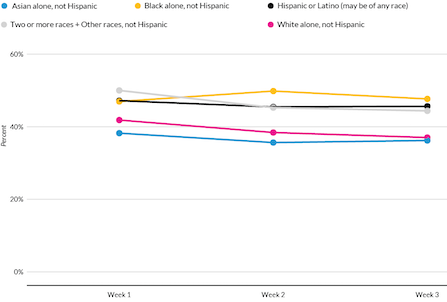
\includegraphics[width=\textwidth, height=0.23\textheight, keepaspectratio]{images/fig_14_15_deficit_chart.png}\\[0.1cm]
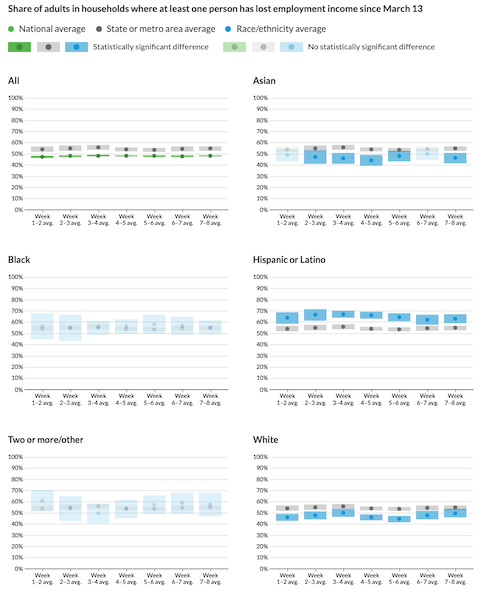
\includegraphics[width=\textwidth, height=0.25\textheight, keepaspectratio]{images/fig_14_16_separate_panels.png}\\[0.08cm]
{\fontsize{6.5pt}{7.8pt}\selectfont \textcolor{navyMuted}{\textit{Hình 14.15: Biểu đồ gộp thiếu hụt vs Hình 14.16: Tách khung công bằng.}}}
\end{column}
\end{columns}
\slidenumber{11}
\end{frame}

% ==================== SLIDE 12: ĐỊNH KIẾN KHÔNG GIAN (1): DIỆN TÍCH & CARTOGRAM ====================


\begin{frame}[plain, t]


\slideheader{Mục 02 • Giảm Thiểu Định Kiến}{Định Kiến Diện Tích, Mercator \& Giải Pháp Cartogram}
\begin{columns}[T]
\begin{column}{0.52\textwidth}
{\fontsize{8.2pt}{10.5pt}\selectfont
\calloutbox[\textwidth]{Nguyên Lý Sống Còn}{
    \textit{``Đất đai không đi bầu cử, con người mới đi bầu!''}
}

\vspace{0.12cm}
\textbf{1. Định kiến Diện tích (Map Area Bias):}
\begin{itemize}\setlength{\itemsep}{1.5pt}
    \item Bang nông thôn Wyoming lớn gấp \textbf{80 lần} Rhode Island nhưng chỉ có $600\text{k dân}$ ($3$ phiếu đại cử tri), trong khi Rhode Island có $>1\text{M dân}$ ($4$ phiếu). Bản đồ thường phóng đại tầm ảnh hưởng các bang ít dân!
\end{itemize}

\vspace{0.12cm}
\textbf{2. Định kiến Phép chiếu (Projection Bias):}
\begin{itemize}\setlength{\itemsep}{1.5pt}
    \item Web Mercator phóng đại Bắc Mỹ/Châu Âu, thu nhỏ Châu Phi.
    \item \textbf{✅ Giải pháp: Bản đồ Cartogram (Lục giác / Ô vuông dân số):} Quy đổi diện tích theo số dân / đại cử tri.
\end{itemize}
}
\end{column}
\begin{column}{0.44\textwidth}
\centering
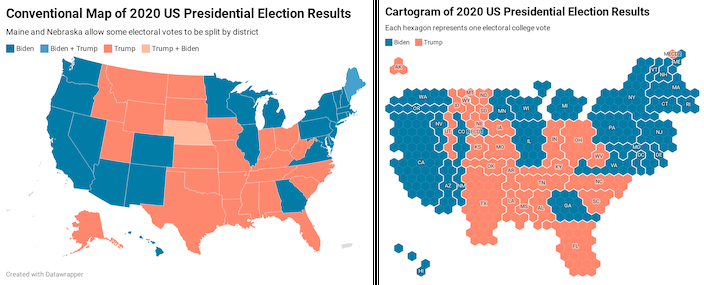
\includegraphics[width=\textwidth, height=0.24\textheight, keepaspectratio]{images/fig_14_17_cartogram_election.png}\\[0.1cm]
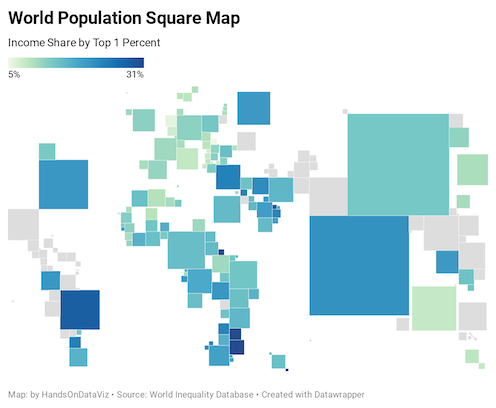
\includegraphics[width=\textwidth, height=0.24\textheight, keepaspectratio]{images/fig_14_18_population_squares.png}\\[0.08cm]
{\fontsize{6.5pt}{7.8pt}\selectfont \textcolor{navyMuted}{\textit{Hình 14.17: Cartogram bầu cử Mỹ \& Hình 14.18: Ô vuông dân số thế giới.}}}
\end{column}
\end{columns}
\slidenumber{12}
\end{frame}

% ==================== SLIDE 13: ĐỊNH KIẾN KHÔNG GIAN (2): TRANH CHẤP & LOẠI TRỪ ====================


\begin{frame}[plain, t]


\slideheader{Mục 02 • Giảm Thiểu Định Kiến}{Định Kiến Lãnh Thổ Tranh Chấp \& Sự Loại Trừ}
\begin{columns}[T]
\begin{column}{0.52\textwidth}
{\fontsize{8.2pt}{10.5pt}\selectfont
\textbf{3. Định kiến Lãnh thổ Tranh chấp (Disputed Territory):}
\begin{itemize}\setlength{\itemsep}{1.5pt}
    \item Google Maps đổi biên giới Crimea tùy IP (ở Nga hiển thị nét liền thuộc Nga; ở ngoài hiển thị nét đứt tranh chấp).
    \item $\rightarrow$ \textit{Giải pháp:} Tham khảo OpenStreetMap, Native Land.
\end{itemize}

\vspace{0.12cm}
\textbf{4. Định kiến Loại trừ trên Bản đồ (Map Exclusion Bias):}
\begin{itemize}\setlength{\itemsep}{1.5pt}
    \item Nhiều bản đồ chỉ vẽ 50 bang và \textbf{bỏ qua Thủ đô Washington D.C.} ($>700\text{k dân}$) và \textbf{Puerto Rico} ($>3\text{M dân}$) cùng các đảo hải ngoại -- nơi đa số là người da màu.
    \item $\rightarrow$ Luôn chọn bản đồ tích hợp đầy đủ lãnh thổ.
\end{itemize}
}
\end{column}
\begin{column}{0.44\textwidth}
\centering
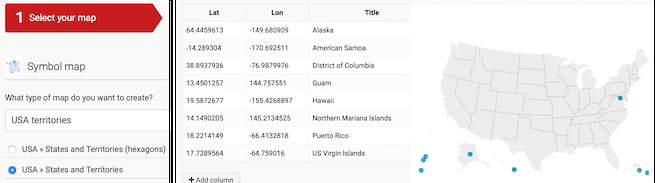
\includegraphics[width=\textwidth, height=0.52\textheight, keepaspectratio]{images/fig_14_19_map_exclusion.png}\\[0.15cm]
{\fontsize{6.8pt}{8pt}\selectfont \textcolor{navyMuted}{\textit{Hình 14.19: Datawrapper hiển thị đầy đủ D.C. và các lãnh thổ hải ngoại.}}}
\end{column}
\end{columns}
\slidenumber{13}
\end{frame}

% ==================== SLIDE 14: CHUYỂN TIẾP MỤC 03 ====================


\begin{frame}[plain, c]


\begin{tikzpicture}[remember picture,overlay]
    \node[anchor=west, text width=0.76\textwidth] at ($(current page.west)+(1.0cm, 0.2cm)$) {
        {\fontsize{13pt}{15pt}\selectfont \textbf{\color{navyMuted} PHẦN 4 • MỤC 03}}\\[0.25cm]
        {\fontsize{28pt}{32pt}\selectfont \textbf{\color{navyMain} NGHỆ THUẬT KỂ CHUYỆN}}\\[0.12cm]
        {\fontsize{22pt}{26pt}\selectfont \textbf{\color{navyMain} DỮ LIỆU}}\\[0.35cm]
        \pillbox{\fontsize{10pt}{12pt}\selectfont Chapter 15: Tell and Show Your Data Story}\\[0.45cm]
        {\normalsize \color{navyMuted} \textit{``Công thức Tell — Show — Why:\\Dẫn dắt nhận thức và thúc đẩy hành động.''}}
    };
\end{tikzpicture}
\slidenumber{14}
\end{frame}

% ==================== SLIDE 15: CÔNG THỨC TELL - SHOW - WHY ====================


\begin{frame}[plain, t]


\slideheader{Mục 03 • Kể Chuyện Dữ Liệu}{Triết Lý Kể Chuyện: ``Tell -- Show -- Why''}
\calloutbox[\textwidth]{Đừng Bắt Khán Giả Tự Đoán Ý Nghĩa!}{
    Biểu đồ không tự lên tiếng -- bạn chính là người dẫn đường chỉ cho khán giả thấy \textbf{``khu rừng tổng thể'' (the forest)} và điểm xuyết \textbf{``một vài cái cây đặc biệt'' (special trees)} làm minh họa.
}

\vspace{0.15cm}
\begin{columns}[T]
\begin{column}{0.31\textwidth}
\calloutbox[\textwidth]{1. TELL (Nói trước)}{
    Tóm tắt thông điệp quan trọng nhất bằng \textbf{1 câu tiêu đề sắc gọn (Headline sentence)} ngay phía trên đồ thị.
}
\end{column}
\begin{column}{0.31\textwidth}
\calloutbox[\textwidth]{2. SHOW (Chiếu bằng chứng)}{
    Đưa ra biểu đồ hoặc bản đồ đã thiết kế trung thực, tinh giản làm \textbf{bằng chứng thị giác thuyết phục} ở giữa.
}
\end{column}
\begin{column}{0.31\textwidth}
\calloutbox[\textwidth]{3. WHY (Hành động)}{
    Giải thích \textbf{tại sao nó quan trọng}: Thay đổi tư duy, chính sách hay thúc đẩy chúng ta \textbf{hành động} như thế nào ở đáy.
}
\end{column}
\end{columns}
\slidenumber{15}
\end{frame}

% ==================== SLIDE 16: BẢNG PHÂN CẢNH DATA STORYBOARD ====================


\begin{frame}[plain, t]


\slideheader{Mục 03 • Kể Chuyện Dữ Liệu}{Xây Dựng Bảng Phân Cảnh (Data Storyboard)}
\begin{columns}[T]
\begin{column}{0.52\textwidth}
{\fontsize{8.2pt}{10.5pt}\selectfont
\textbf{4 Bước phác thảo kịch bản (Sketch Your Data Story):}
\begin{enumerate}\setlength{\itemsep}{1.5pt}
    \item Xác định \textbf{Vấn đề thực tiễn (Problem)} thúc đẩy dự án.
    \item Chuyển hóa thành \textbf{Câu hỏi nghiên cứu (Question)}.
    \item Kế hoạch \textbf{Tìm kiếm \& thu thập dữ liệu (Find Data)}.
    \item Phác thảo \textbf{Ý tưởng trực quan hóa (Visualize)}.
\end{enumerate}

\vspace{0.12cm}
\textbf{3 Lời khuyên vàng tránh lỗi kịch bản:}
\begin{itemize}\setlength{\itemsep}{1.5pt}
    \item Luôn nêu Vấn đề trước khi đưa ra Đáp án.
    \item Tóm tắt Luận điểm (Insight) trước khi chiếu đồ thị.
    \item Đảm bảo Câu hỏi ban đầu và Kết luận cuối cùng khớp nhau!
\end{itemize}
}
\end{column}
\begin{column}{0.44\textwidth}
\centering
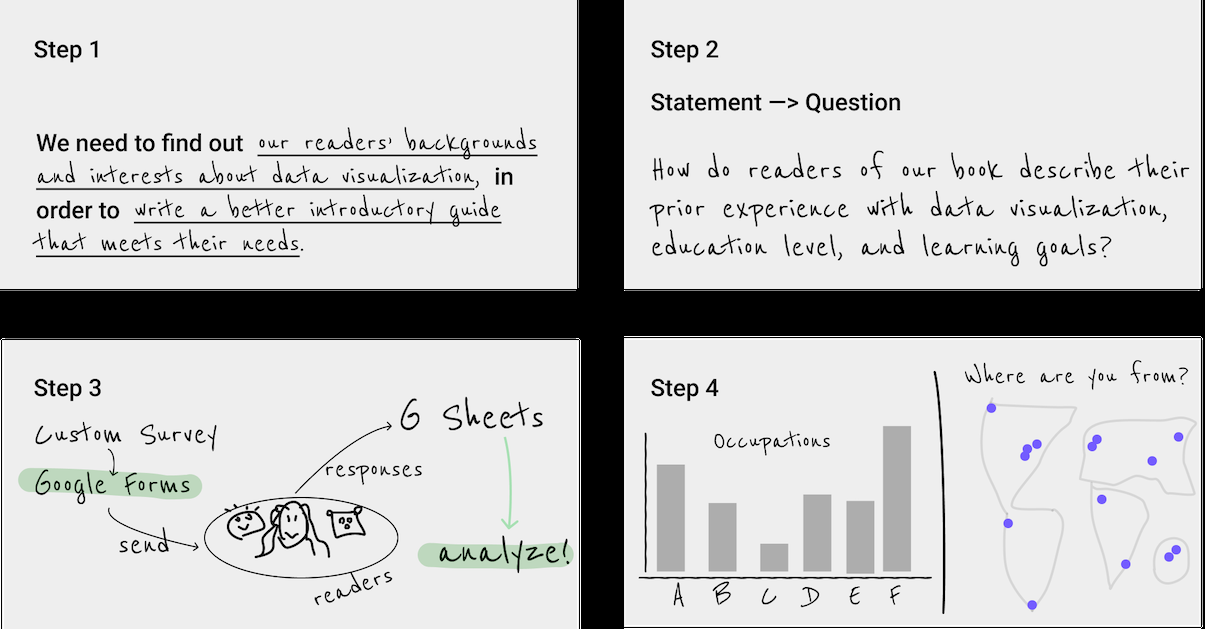
\includegraphics[width=\textwidth, height=0.23\textheight, keepaspectratio]{images/fig_15_1_storyboard_sketch.png}\\[0.1cm]
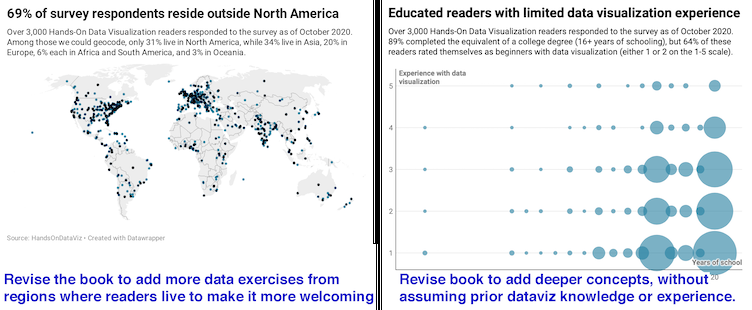
\includegraphics[width=\textwidth, height=0.25\textheight, keepaspectratio]{images/fig_15_2_tell_show_why.png}\\[0.08cm]
{\fontsize{6.5pt}{7.8pt}\selectfont \textcolor{navyMuted}{\textit{Hình 15.1: Phác thảo Storyboard \& Hình 15.2: Cấu trúc Tell-Show-Why.}}}
\end{column}
\end{columns}
\slidenumber{16}
\end{frame}

% ==================== SLIDE 17: MÀU SẮC & CHÚ THÍCH (CASE STUDY NHỰA) ====================


\begin{frame}[plain, t]


\slideheader{Mục 03 • Kể Chuyện Dữ Liệu}{Màu Sắc \& Chú Thích Trực Tiếp (Case Study Nhựa)}
\begin{columns}[T]
\begin{column}{0.52\textwidth}
{\fontsize{8.2pt}{10.5pt}\selectfont
\textbf{Sản lượng Nhựa Toàn cầu 1950--2015 (Our World In Data):}

\vspace{0.12cm}
\textbf{1. Biểu đồ đường mặc định (Hình 15.3):}
\begin{itemize}\setlength{\itemsep}{1.5pt}
    \item Chỉ thấy sản lượng tăng đều theo năm $\rightarrow$ Nhạt nhòa, thiếu điểm nhấn!
\end{itemize}

\vspace{0.12cm}
\textbf{2. Khám phá lớn \& Tái thiết kế thành Area Chart (Hình 15.5):}
\begin{itemize}\setlength{\itemsep}{1.5pt}
    \item \textbf{Phát hiện chấn động:} Hơn một nửa (\textbf{59\%}) lượng nhựa từng được sản xuất trong toàn bộ lịch sử nhân loại mới chỉ được tạo ra \textbf{từ năm 2000 trở lại đây}!
    \item Tách 2 cột trước/sau 2000 $\rightarrow$ Chuyển sang \textbf{Area Chart} thể hiện tổng tích lũy $\rightarrow$ Tô xám quá khứ, tô \textbf{xanh đậm nổi bật từ 2000} kèm chú thích \texttt{59\%} ngay trong hình!
\end{itemize}
}
\end{column}
\begin{column}{0.44\textwidth}
\centering
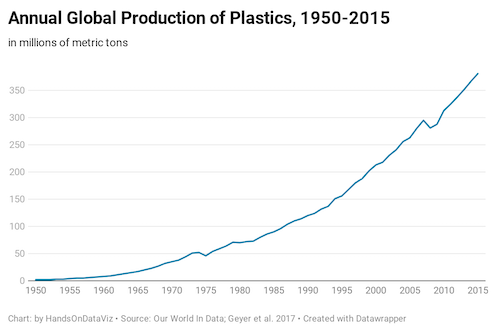
\includegraphics[width=\textwidth, height=0.23\textheight, keepaspectratio]{images/fig_15_3_plastics_line.png}\\[0.1cm]
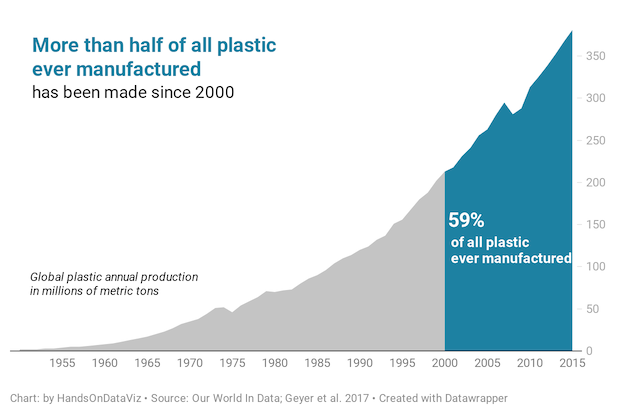
\includegraphics[width=\textwidth, height=0.25\textheight, keepaspectratio]{images/fig_15_5_plastics_annotated.png}\\[0.08cm]
{\fontsize{6.5pt}{7.8pt}\selectfont \textcolor{navyMuted}{\textit{Hình 15.3: Line chart mặc định vs Hình 15.5: Area chart chú thích 59\%.}}}
\end{column}
\end{columns}
\slidenumber{17}
\end{frame}

% ==================== SLIDE 18: MINH BẠCH, BẤT ĐỊNH & ĐỊNH DẠNG MỚI ====================


\begin{frame}[plain, t]


\slideheader{Mục 03 • Kể Chuyện Dữ Liệu}{Minh Bạch Sự Bất Định \& Định Dạng Kể Chuyện Mới}
\begin{columns}[T]
\begin{column}{0.52\textwidth}
{\fontsize{7.8pt}{9.8pt}\selectfont
\textbf{4 Nguyên tắc xây dựng uy tín (Credibility):}
\begin{enumerate}\setlength{\itemsep}{1pt}
    \item Trình bày trung thực, cảnh báo suy diễn quá đà.
    \item Ghi rõ liên kết nguồn (Source links) \& cộng sự (Credits).
    \item Lưu trữ quy trình làm sạch (GitHub) để có thể tái lập.
    \item \textbf{Thừa nhận bất định (Disclose Uncertainty):} Vẽ \textbf{Đường nét liền (Solid line)} cho dữ liệu thực tế quan sát và \textbf{Đường nét đứt (Dashed line)} cho dữ liệu dự báo tương lai.
\end{enumerate}

\vspace{0.08cm}
\textbf{Các định dạng kể chuyện hiện đại:}
\begin{itemize}\setlength{\itemsep}{1pt}
    \item \textbf{Web tương tác:} Nhúng iframe biểu đồ động.
    \item \textbf{Video Screencast:} Quay màn hình tương tác có lồng tiếng.
    \item \textbf{Data Walk:} In biểu đồ khổ lớn triển lãm cộng đồng.
\end{itemize}
}
\end{column}
\begin{column}{0.44\textwidth}
\centering
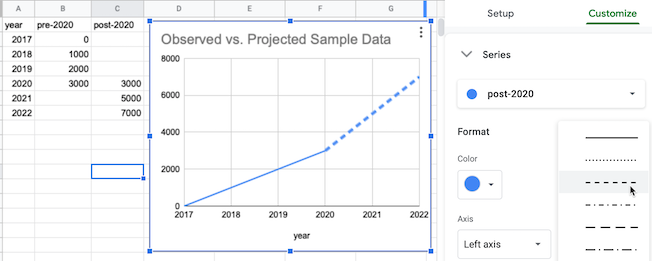
\includegraphics[width=\textwidth, height=0.52\textheight, keepaspectratio]{images/fig_15_6_observed_vs_projected.png}\\[0.15cm]
{\fontsize{6.8pt}{8pt}\selectfont \textcolor{navyMuted}{\textit{Hình 15.6: Tách cột để vẽ nét liền (Observed) nối nét đứt (Projected).}}}
\end{column}
\end{columns}
\slidenumber{18}
\end{frame}

% ==================== SLIDE 19: TỔNG KẾT TOÀN BỘ HÀNH TRÌNH ====================


\begin{frame}[plain, t]


\slideheader{Tổng Kết Toàn Bộ}{Từ Dữ Liệu Thô Đến Câu Chuyện Truyền Cảm Hứng}
\begin{columns}[T]
\begin{column}{0.24\textwidth}
\begin{tikzpicture}
    \node[draw=navyMain, fill=boxBg, rounded corners=5pt, line width=0.8pt, inner sep=5pt, text width=\textwidth-12pt, align=left] {
        {\fontsize{8pt}{10pt}\selectfont \textbf{\color{navyMain} PHẦN 1}}\\[0.03cm]
        {\fontsize{6.8pt}{8.2pt}\selectfont \color{navyMuted} Nền Tảng Dữ Liệu}\\[0.08cm]
        {\fontsize{6.5pt}{8pt}\selectfont \color{navyMain}
        • Săn tìm có định hướng\\
        • Bảo mật Masking/Agg.\\
        • Làm sạch bẩn \& bẫy chuỗi\\
        • So sánh Median, VMT}
    };
\end{tikzpicture}
\end{column}
\begin{column}{0.24\textwidth}
\begin{tikzpicture}
    \node[draw=navyMain, fill=boxBg, rounded corners=5pt, line width=0.8pt, inner sep=5pt, text width=\textwidth-12pt, align=left] {
        {\fontsize{8pt}{10pt}\selectfont \textbf{\color{navyMain} PHẦN 2}}\\[0.03cm]
        {\fontsize{6.8pt}{8.2pt}\selectfont \color{navyMuted} Trực Quan Biểu Đồ}\\[0.08cm]
        {\fontsize{6.5pt}{8pt}\selectfont \color{navyMain}
        • Gốc 0 cho Cột/Thanh\\
        • Tổng 100\% cho Pie 12h\\
        • Loại bỏ rác đồ họa 3D\\
        • Range, Scatter, Bubble}
    };
\end{tikzpicture}
\end{column}
\begin{column}{0.24\textwidth}
\begin{tikzpicture}
    \node[draw=navyMain, fill=boxBg, rounded corners=5pt, line width=0.8pt, inner sep=5pt, text width=\textwidth-12pt, align=left] {
        {\fontsize{8pt}{10pt}\selectfont \textbf{\color{navyMain} PHẦN 3}}\\[0.03cm]
        {\fontsize{6.8pt}{8.2pt}\selectfont \color{navyMuted} Bản Đồ Không Gian}\\[0.08cm]
        {\fontsize{6.5pt}{8pt}\selectfont \color{navyMain}
        • Phân biệt Point/Polygon\\
        • 1 biến duy nhất\\
        • Bảng màu ColorBrewer\\
        • Chuẩn hóa Choropleth}
    };
\end{tikzpicture}
\end{column}
\begin{column}{0.24\textwidth}
\begin{tikzpicture}
    \node[draw=navyMain, fill=boxBg, rounded corners=5pt, line width=0.8pt, inner sep=5pt, text width=\textwidth-12pt, align=left] {
        {\fontsize{8pt}{10pt}\selectfont \textbf{\color{navyMain} PHẦN 4}}\\[0.03cm]
        {\fontsize{6.8pt}{8.2pt}\selectfont \color{navyMuted} Đạo Đức \& Kể Chuyện}\\[0.08cm]
        {\fontsize{6.5pt}{8pt}\selectfont \color{navyMain}
        • Phát hiện mánh khóe lừa\\
        • Khắc phục định kiến Carto\\
        • Công thức Tell-Show-Why\\
        • Minh bạch sự bất định}
    };
\end{tikzpicture}
\end{column}
\end{columns}
\vspace{0.35cm}
\centering
\pillbox{\fontsize{10pt}{12pt}\selectfont THANK YOU FOR WATCHING! — Q\&A}
\slidenumber{19}
\end{frame}


\end{document}
